\documentclass[a4paper]{article}

\usepackage{amsmath}
\usepackage{amssymb}
\usepackage[margin=1.5cm,
            includefoot,
            footskip=30pt]{geometry}
\usepackage{layout}
\usepackage{graphicx}

\usepackage{biblatex}

\bibliography{main.bib}



\title{Comparison of steady states}
\author{}
\date{}

\begin{document}

\maketitle

Using the pair wise interactions the transition rates \(p,
q\) can be measured and the steady state probabilities inferred and compared to
the actual probabilities of each state.
This is done numerically by computing the singular eigenvector of the
matrix \(A\) \cite{Stewart2009}:

\[
    A =
    \begin{bmatrix}
        p_1 q_1 & p_1 (1 - q_1) & (1 - p_1) q_1 & (1 -p_1) (1 - q_1) \\
        p_2 q_2 & p_2 (1 - q_2) & (1 - p_2) q_2 & (1 -p_2) (1 - q_2) \\
        p_3 q_3 & p_3 (1 - q_3) & (1 - p_3) q_3 & (1 -p_3) (1 - q_3) \\
        p_4 q_4 & p_4 (1 - q_4) & (1 - p_4) q_4 & (1 -p_4) (1 - q_4) \\
    \end{bmatrix}
\]

Figure~\ref{fig:computed_probabilities_vs_theoretic_probabilities} shows a
regression line fitted to every pairwise interaction with a reported
\(\text{SSError}\) value (pairwise interactions with missing states were
omitted). This serves to validate the approach: a part from some edge cases the
relationship is consistent.

\begin{figure}[!htbp]
    \centering
    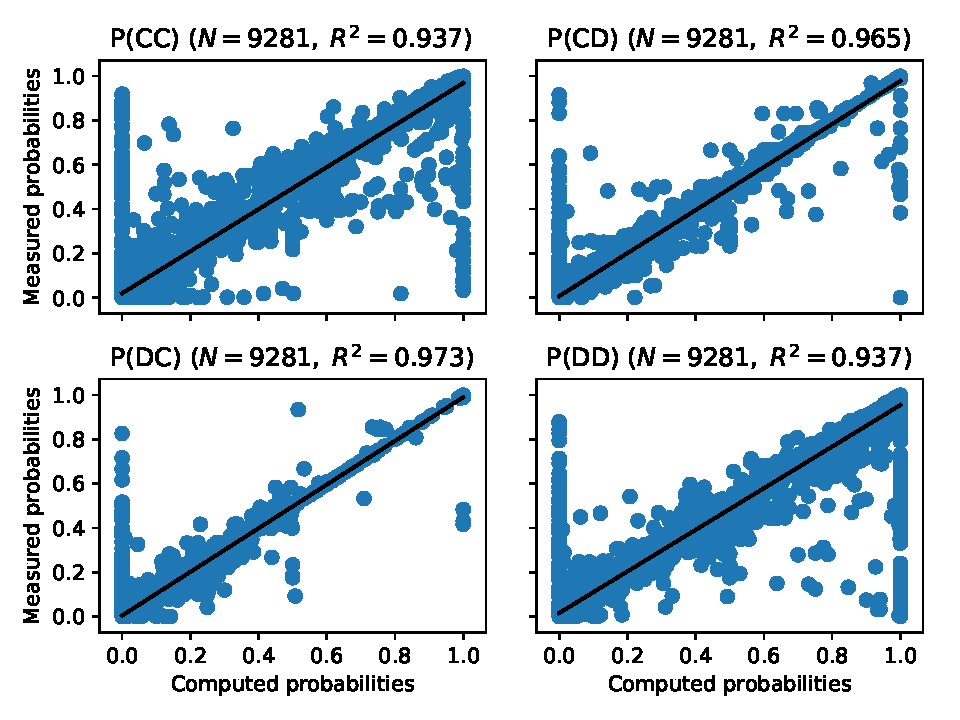
\includegraphics[width=.8\textwidth]{../../img/computed_probabilities_vs_theoretic_probabilities/main.pdf}
    \caption{The
        relationship between the steady state probabilities inferred from the
        measured transitions and the actual steady state probabilities. A linear
        regression line is included validating the approach.}
    \label{fig:computed_probabilities_vs_theoretic_probabilities}
\end{figure}


\printbibliography

\end{document}
